\section{Implementazione}

\subsection{Basis1DAbstract}

\begin{frame}
\tableofcontents[currentsection]
\end{frame}

\begin{frame}
 \frametitle{Basis1DAbstract}
 \framesubtitle{Una classe astratta per risolvere i sottoproblemi agli autovalori}
 \begin{columns}
  \begin{column}{0.5\textwidth}
  Il problema viene sempre rimappato nell'intervallo $(0,1)$
 \begin{itemize}
  \item Calcola gli autovalori\\$\rightarrow$ \texttt{Next()}
  \item Valuta le funzioni di base\\$\rightarrow$ \texttt{EvaluateBasis(...)}
 \end{itemize}
  \end{column}
\begin{column}{0.5\textwidth}
 \begin{figure}
  \centering
  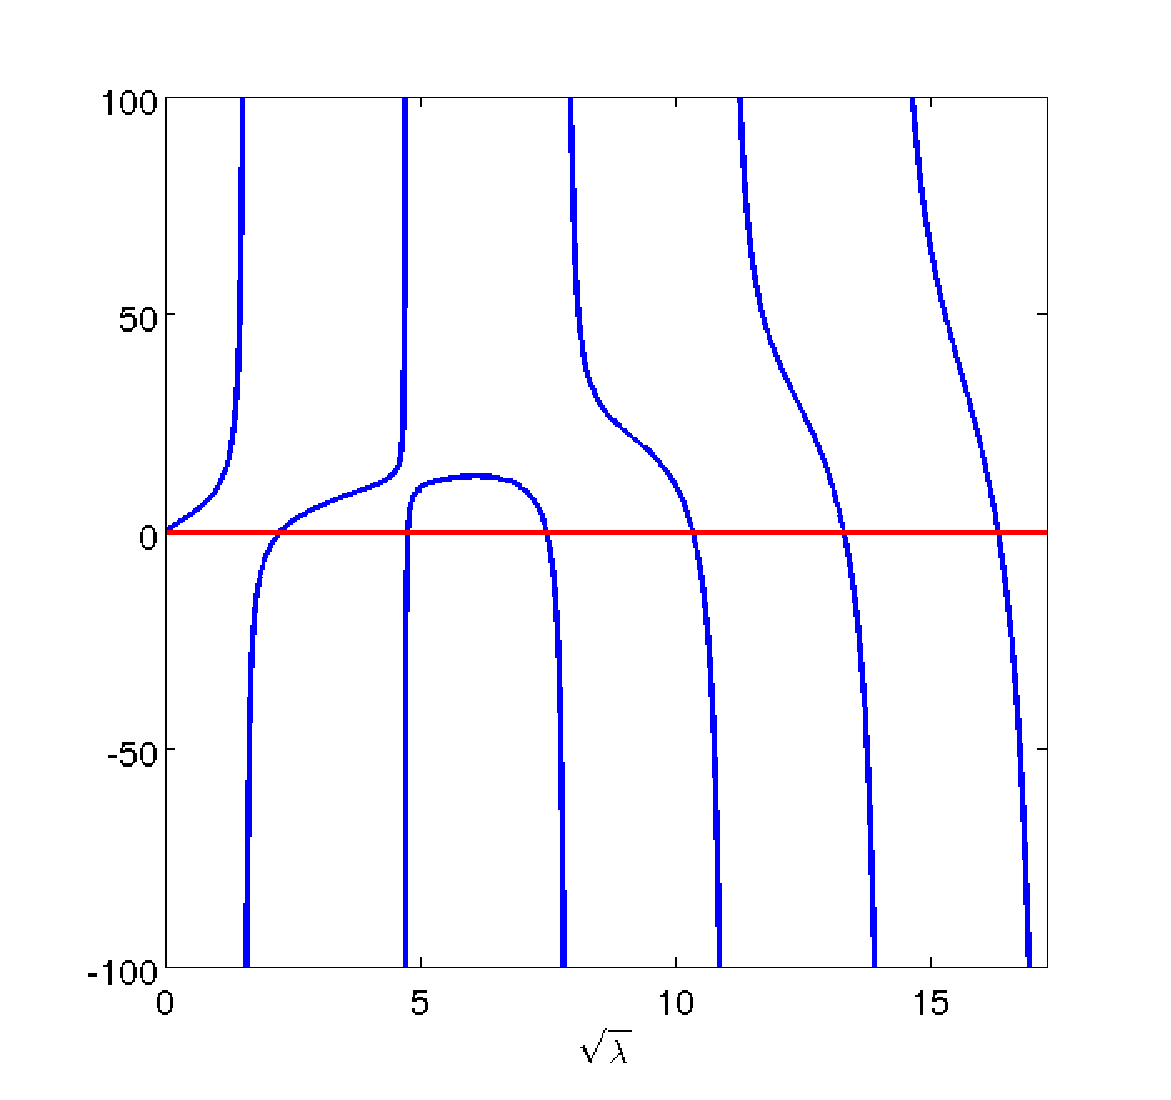
\includegraphics[scale=0.3,trim=1cm 1cm 1cm 1cm,clip=true]{Varie/ricercazeri}
 \end{figure}
\begin{center}Ricerca degli zeri con condizioni di Robin\end{center}
\end{column}
 \end{columns}
\end{frame}
\begin{frame}
 \frametitle{Polimorfismo su \texttt{Basis1DAbstract}...}
 \framesubtitle{... e su \texttt{EducatedBasisFunctorAbstract}}
 \begin{columns}
  \begin{column}{0.5\textwidth}
 \begin{figure}
  \centering
  {\linkimage{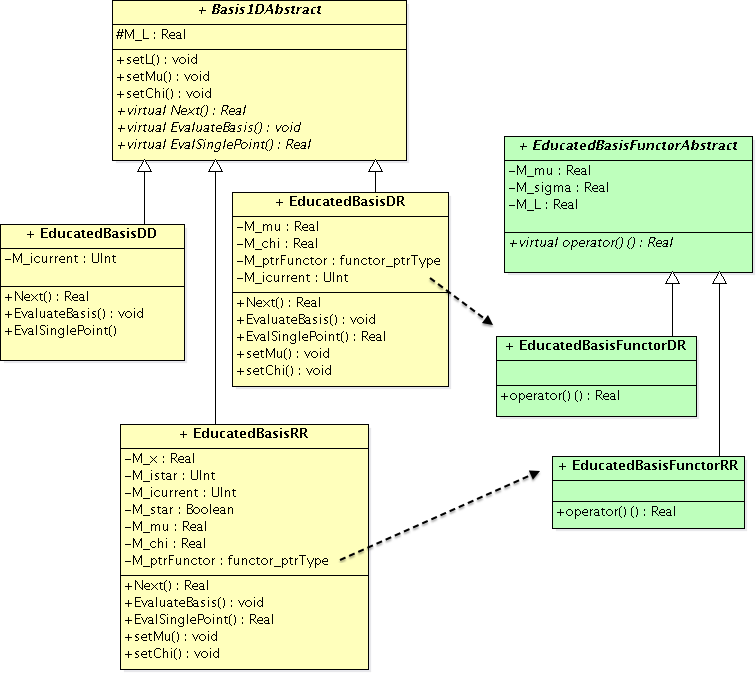
\includegraphics[scale=0.2]{UML/Basis1DAbstract}}{UML/Basis1DAbstract}}
 \end{figure}
  \end{column}
  \begin{column}{0.5\textwidth}
   Per gestire le diverse classi figlie di \texttt{Basis1DAbstract} abbiamo utilizzato una \textbf{factory}.
  \end{column}
 \end{columns}
\end{frame}

\subsection{ModalSpace}

\begin{frame}
\tableofcontents[currentsection]
\end{frame}

\begin{frame}
 \frametitle{\texttt{ModalSpace}}
 \framesubtitle{Una classe che gestisce la costruzione dell'intera base modale}
 \begin{itemize}
  \item Gestisce le formule di quadratura sulla slice
  \item Istanzia i corretti generatori di base\\
  $\rightarrow$ \texttt{AddSliceBC(...)}
  \item Calcola gli autovalori del problema 2D\\
  $\rightarrow$ \texttt{EigensProvider(...)}
  \item Valuta le funzioni di base e le loro derivate nei nodi di quadratura\\
  $\rightarrow$ \texttt{EvaluateBasis(...)}
  \item Calcola i coefficient $r^{st}_{k,j}$\\
  $\rightarrow$ \texttt{Compute\_*(...)}
 \end{itemize}
\end{frame}
\begin{frame}[fragile]
\frametitle{\texttt{AddSliceBC(...)}}
\framesubtitle{due metodi uno per ogni direzione}
\begin{lstlisting}[style = general]
void ModalSpace::
AddSliceBCY (const string& left, const string& right, const Real& mu, const Real& chi)
{
	// Creation of the correct basis generator
	M_genbasisY = Basis1DFactory::istance().createObject(left+right);
	// Setting of the parameters
	M_genbasisY->setL(M_Ly);
	M_genbasisY->setMu(mu);
	M_genbasisY->setChi(chi);
	return;
}
\end{lstlisting}
\end{frame}

\begin{frame}
\frametitle{EigensProvider()}
\framesubtitle{Ordinare correttamente gli autovalori non \`e facile}
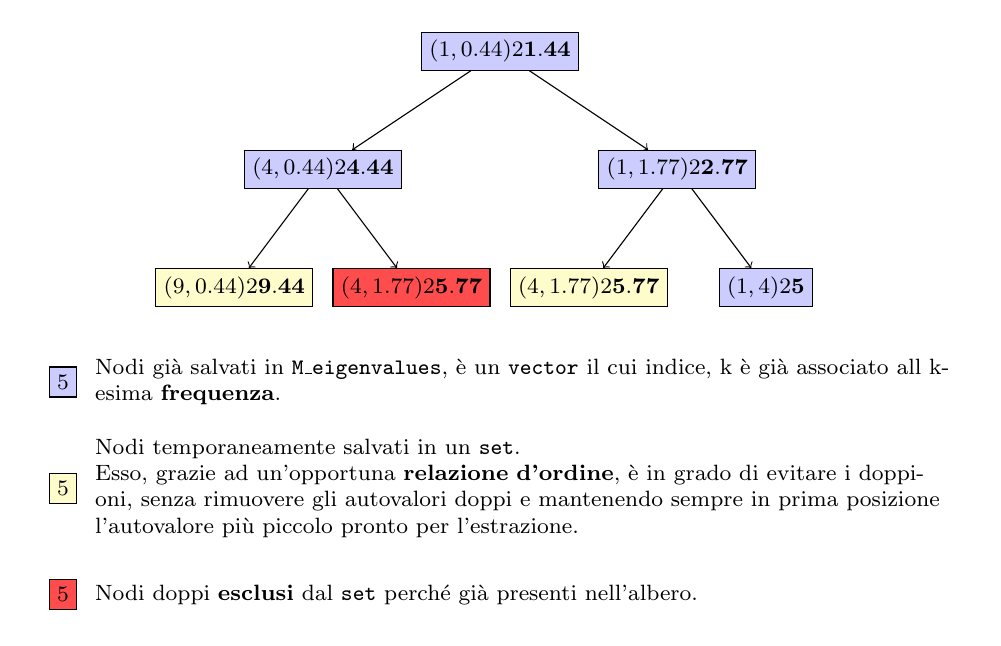
\begin{tikzpicture}
[scale=1.5]
\footnotesize
\tikzstyle{eig}=[rectangle, draw, fill=blue!20];
\tikzstyle{temp}=[rectangle,draw,fill=yellow!20];
\tikzstyle{rip}=[rectangle,draw,fill=red!70];
\def\yo{4.8}
\def\dy{-1}
\def\c{1.5}
\def\spazio{2}
\useasboundingbox (-4,0) rectangle (4,5);
\node<1->[eig] (v1) at (0,\yo)  {$(1,0.44)\psp{\spazio}\mathbf{1.44}$};
\node<2-4>[temp] (v2) at (-\c,\yo+\dy)  {$(4,0.44)\psp{\spazio}\mathbf{4.44}$};
\node<2-2>[temp] (v3) at (+\c,\yo+\dy)   {$(1,1.77)\psp{\spazio}\mathbf{2.77}$};
\draw<2->[->] (v1) -- (v2);
\draw<2->[->] (v1) -- (v3);
\node<3->[eig] (v3) at (+\c,\yo+\dy)   {$(1,1.77)\psp{\spazio}\mathbf{2.77}$};
\node<4->[temp] (v4) at (\c - \c/2,\yo+2*\dy) {$(4,1.77)\psp{\spazio}\mathbf{5.77}$};
\node<4-8>[temp] (v5) at (\c + \c/2,\yo+2*\dy) {$(1,4)\psp{\spazio}\mathbf{5}$};
\draw<4->[->] (v3) -- (v4);
\draw<4-8>[->] (v3) -- (v5);
\node<5->[eig] (v2) at (-\c,\yo+\dy) {$(4,0.44)\psp{\spazio}\mathbf{4.44}$};
\node<6->[temp] (v6) at (-\c-\c/2,\yo+2*\dy) {$(9,0.44)\psp{\spazio}\mathbf{9.44}$};
\node<6-6>[temp] (v7) at (-\c+\c/2,\yo+2*\dy) {$(4,1.77)\psp{\spazio}\mathbf{5.77}$};
\draw<6->[->] (v2) -- (v6);
\draw<6->[->] (v2) -- (v7);
\node<7->[rip] (v7) at (-\c+\c/2,\yo+2*\dy) {$(4,1.77)\psp{\spazio}\mathbf{5.77}$};
\node<8->[eig] (v5) at (\c + \c/2,\yo+2*\dy) {$(1,4)\psp{\spazio}\mathbf{5}$};

\def\s{-0.5}
\def\sp{0.3}
\node<1->[eig] (legeig) at (-4+\sp,\s+\yo+2.3*\dy) {$\psp{5}$};
\node<1->[right,text width=11.5cm] (texteig) at (-3.5,\s+\yo+2.3*\dy) {Nodi gi\`a salvati in \texttt{M\_eigenvalues}, 
\`e un \texttt{vector} il cui indice, k \`e gi\`a associato all k-esima \textbf{frequenza}.};
\node<2->[temp] (legtmp) at (-4+\sp,\s+\yo+3.2*\dy) {$\psp{5}$};
\node<2->[right,text width=11.5cm] (texteig) at (-3.5,\s+\yo+3.2*\dy) {Nodi temporaneamente salvati in un \texttt{set}.\\ Esso, grazie ad un'%
opportuna \textbf{relazione d'ordine}, \`e in grado di evitare i doppioni, senza rimuovere gli autovalori doppi e mantenendo 
sempre in prima posizione l'autovalore pi\`u piccolo pronto per l'estrazione.};
\node<7->[rip] (legrip) at (-4+\sp,\s+\yo+4.1*\dy) {$\psp{5}$};
\node<7->[right,text width=11.5cm] (texteig) at (-3.5,\s+\yo+4.1*\dy) {Nodi doppi \textbf{esclusi} dal \texttt{set} perch\'e gi\`a presenti nell'albero.};
\end{tikzpicture}
\end{frame}

\begin{frame}[fragile]
\frametitle{\texttt{EvaluateBasis(...)}}
\framesubtitle{Valutare le funzioni di base sui nodi di quadratura}
\begin{lstlisting}[style=general]
void ModalSpace::
EvaluateBasis()
{
    // Compute all the eigens from the 1D problems
    EigensProvider();
    
    // Fill the matrices with the evaluation of 
    // the monodimensional basis and its derivatives
    M_genbasisY->EvaluateBasis (M_phiy, M_dphiy, 
                                M_eigenvaluesY, M_quadruleY);
    M_genbasisZ->EvaluateBasis (M_phiz, M_dphiz, 
                                M_eigenvaluesZ, M_quadruleZ);
}
\end{lstlisting}
\end{frame}
\begin{frame}[fragile]
 \frametitle{\texttt{Compute\_*(..)}}
 \framesubtitle{Sfruttando la separazione di variabili}
 \begin{lstlisting}[style=general]
Real ModalSpace::
Compute_PhiPhi (const UInt& j, const UInt& k) const
{   //... 
    //... (Date le frequenze estrae i sottoindici p e q)
    for (UInt n = 0; n < M_quadruleY->nbQuadPt(); ++n)
    coeff_y += M_phiy [p_j][n] * normy *
                   M_phiy [p_k][n] * normy *
                   M_Ly * M_quadruleY->weight (n);
    for (UInt n = 0; n < M_quadruleZ->nbQuadPt(); ++n)
    coeff_z += M_phiz[q_j][n] * normz *
                   M_phiz[q_k][n] * normz *
                   M_Lz * M_quadruleZ->weight (n);
    return coeff_y * coeff_z;
}
\end{lstlisting}

{\footnotesize\textbf{\red{WIP}}: Abbiamo aggiunto dei metodi per considerare 
\textbf{coefficienti non costanti} che si occupano di calcolare i coefficienti $r^{st}_{j,k}$ \textbf{senza separare le variabili}.

Sono ancora da testare e da ottimizzare.}
\end{frame}

\subsection{HiModAssembler}

\begin{frame}
\tableofcontents[currentsection]
\end{frame}

\begin{frame}
 \frametitle{HiModAssembler}
 \framesubtitle{La classe che combina gli elementi finiti e la base modale}
 \begin{itemize}
  \item \textbf{Membri principali}
  \begin{itemize}
   \item \texttt{M\_modalbasis}
   \item \texttt{M\_etfespace}
  \end{itemize}

  \item Metodi per l'\textbf{assemblaggio}
  \begin{itemize}
   \item \texttt{AddADRProblem(...)}
   \item \texttt{interpolate(...)}
   \item \texttt{Addrhs(...)}
   \item \texttt{AddDirichletBC\_In(...)}
  \end{itemize}

  \item Metodi per l'\textbf{analisi}
  \begin{itemize}
   \item \texttt{evaluateBase3DGrid(...)} \textcolor{green!50!black}{$//$HiMod vector}
   \item \texttt{evaluateBase3DGrid(...)} \textcolor{green!50!black}{$//$Function type}
   \item \texttt{normL2(...)}
  \end{itemize}

  \item Metodi per l'\textbf{export}
  \begin{itemize}
   \item \texttt{ExportStructuredVTK(...)}
   \item \texttt{ExportFunctionVTK(...)}
  \end{itemize}

 \end{itemize}

\end{frame}
\begin{frame}[fragile]
 \frametitle{\texttt{AddADRProblem(...)}}
 \framesubtitle{Utilizzo del pacchetto ETA per assemblare i problemi 1D}
 \begin{lstlisting}[style=general]
for j {
for k {
VectorSmall<5> Coeff;
Coeff[0] = M_modalbasis->Compute_PhiPhi (j, k);
//...
{ using namespace ExpressionAssembly;
  //...
  integrate(
      elements(M_etfespace->mesh()),
      M_fespace->qr(),
      M_etfespace,
      M_etfespace,
      mu*Coeff[0]*dot(grad(phi_i),grad(phi_j))
      //...
      )
  >>(systemMatrix->block(k,j));
}
//...
return;
\end{lstlisting}
\end{frame}